%
% Zusammenfassung Image Analysis & Computer Vision D-ITET
% ===========================================================================
% Author:			Marco Dober
% Version:			0.1
% Last changed: 	19.09.2019	
% ---------------------------------------------------------------------------

\documentclass[a4paper, fontsize=8pt, landscape, DIV=1]{scrartcl}
\usepackage{lastpage}
\usepackage{hyperref, makecell}
\usepackage[graphicx]{realboxes}
% Include general settings and customized commands
%
% General packages and settings
% ===========================================================================
% Author:			Silvano Cortesi (cortesis@student.ethz.ch)
% Version:			1.2
% Last changed:		03.01.2018
%
% ---------------------------------------------------------------------------




\usepackage[german,british]{babel} %choose your language \usepackage[german]{babel}
%\usepackage[T1]{fontenc}
\usepackage[utf8]{inputenc}
\usepackage{fancyhdr}
%\usepackage{lastpage}
%\usepackage{lmodern}
\usepackage{enumerate}
%\usepackage{float} % for positioning of figures
\usepackage[landscape, margin=1cm]{geometry}
\usepackage[dvipsnames]{xcolor}
\usepackage{pdfpages}


%% Math %%
\usepackage{amscd}
\usepackage{blindtext}
\usepackage{enumitem}
\usepackage{multicol}
\usepackage{parskip}
\usepackage{empheq}
\usepackage{amsmath}
\usepackage{amsfonts}
\usepackage{amssymb}
\usepackage{amsthm}
%\usepackage{adjustbox}
%\usepackage{dsfont}
%\usepackage{esint} % provides \oiint
\usepackage{mathrsfs}
%\usepackage{trfsigns}
%\numberwithin{equation}{subsection}
%\usepackage{numprint}

%% Graphics & Charts %%
\usepackage{graphicx}
%\usepackage{pdfpages}
%\usepackage{booktabs}
%\usepackage{array}
%\usepackage{paralist}
%\usepackage{framed}
%\usepackage{trfsigns}
\usepackage{tikz}
\usepackage{wrapfig}
%\usepackage[lofdepth,lotdepth]{subfig}
%\usepackage{tikz}  %Graphen zeichnen
%\usetikzlibrary{decorations.pathmorphing}
%\usetikzlibrary{arrows.meta,arrows}
%\usepackage{pgfplots}

%% General Settings %%
%\setlength{\parindent}{0px}
%\setkomafont{captionlabel}{\normalfont\bfseries}

%\pagestyle{fancy}
%\lfoot{\tiny \today}
%\rfoot{\thepage\  / \pageref{LastPage}}
%\cfoot{}
%\renewcommand{\footrulewidth}{0.4pt}

%% provides command \uline{} for underlining words
%\usepackage{ulem}

%% colour headings
%\usepackage{color}
%\definecolor{bluen}{cmyk}{1,0.5,0,0}
%\definecolor{bloodorange}{cmyk}{0,.92,1,.2}
%\addtokomafont{section}{\color{bloodorange}}
%\addtokomafont{subsection}{\color{bloodorange}}
%\addtokomafont{subsubsection}{\color{bloodorange}}
%\addtokomafont{paragraph}{\small\color{bloodorange}}
%\addtokomafont{subparagraph}{\small\color{bloodorange}}

%% Signs & Special Formating %%
%\usepackage{ulem} %normalem: \emph{Text} is italic again.
%\usepackage{multicol,multirow}
%\usepackage{tabularx}
%\usepackage{stackrel}
%\usepackage{makeidx}
%\usepackage{mparhack} % bessere margiale bei seitenumbruch

% make document compact
%\usepackage[compact]{titlesec}
%\titlespacing{\section}{0pt}{*1}{*1}
%\titlespacing{\subsection}{0pt}{*1}{*1}
%\titlespacing{\subsubsection}{0pt}{*1}{*1}

\RedeclareSectionCommand[
	%runin=false,
	%afterindent=false,
	beforeskip=3pt,
	afterskip=3pt]{section}
\RedeclareSectionCommand[
	%runin=false,
	%afterindent=false,
	beforeskip=0pt,
	afterskip=2pt]{subsection}
\RedeclareSectionCommand[
	%runin=false,
	%afterindent=false,
	beforeskip=0pt,
	afterskip=1pt]{subsubsection}

\parindent 0pt
\pagestyle{empty}
\setlength{\unitlength}{1cm}
\setlist{leftmargin = *}

%include also newer PDF
\pdfminorversion=6

% Set the color of your style
% Avaiable are: Apricot, Aquamarine, Bittersweet, Black, Blue, blue, BlueGreen, BlueViolet, BrickRed, Brown, BurntOrange, CadetBlue, CarnationPink, Cerulean, CornflowerBlue, Cyan, Dandelion, DarkOrchid, Emerald, ForestGreen, Fuchsia, Goldenrod, Gray, Green, GreenYellow, JungleGreen, Lavender, ... (more at: http://en.wikibooks.org/wiki/LaTeX/Colors)
\def\StyleColor{BrickRed}

%
% General commands
% ===========================================================================
% Author:			Silvano Cortesi (cortesis@student.ethz.ch)
% Version:			1.2
% Last changed:		03.01.2018
%
% ---------------------------------------------------------------------------

%..ROEMISCHE_ZAHLEN
	\newcommand{\Roe}[1]{\uppercase\expandafter{\romannumeral #1 }}

%..ZAHLENMENGEN
	\newcommand{\N}{\mathbb{N}}
	\newcommand{\Z}{\mathbb{Z}}
	\newcommand{\Q}{\mathbb{Q}}
	\newcommand{\R}{\mathbb{R}}
	\newcommand{\real}{\R}
	\newcommand{\C}{\mathbb{C}}
	\newcommand{\complex}{\C}
	\newcommand{\0}{\mathbb{O}}
	\newcommand{\F}{\mathbb{F}}
	\newcommand{\K}{\mathbb{K}}
    \newcommand{\angstrom}{\textup{\AA}}
    
%..PFEILE
	\renewcommand{\leadsto}{\Longrightarrow}
	\newcommand{\leftrightleadsto}{\Longleftrightarrow}

%..VEKTOREN
	\newcommand{\Ul} {\underline}
	\newcommand{\vEx} {\vec{e}_x}
	\newcommand{\vEy} {\vec{e}_y}
	\newcommand{\vEz} {\vec{e}_z}
	\newcommand{\vEq} {\vec{e_1}}
	\newcommand{\vEw} {\vec{e_2}}
	\newcommand{\vEe} {\vec{e_3}}
	\newcommand{\transpose} {^{\text{T}}}
	\newcommand{\vect}[1]{\boldsymbol{#1}}
	
%..MATRIX
    \newcommand{\MATR}[1]{ \displaystyle \left( \begin{matrix} #1 \end{matrix} \right)}
    \newcommand{\MATRABS}[1]{ \displaystyle \left| \begin{matrix} #1 \end{matrix} \right|}


%..KOMPLEXE ZAHLEN
	\renewcommand{\Re}{\text{Re}\,}
	\renewcommand{\Im}{\text{Im}\,}

%..OPERATOREN
	\DeclareMathOperator{\grad}{grad}
	\renewcommand{\div}{\text{div}\,}
    	\DeclareMathOperator{\rot}{rot}
    	\DeclareMathOperator{\divg}{div}
    	\DeclareMathOperator{\Tr}{Tr}
    	\DeclareMathOperator{\const}{const}
	\DeclareMathOperator{\imag}{i}
	\newcommand{\Lapl}{\hbox{\footnotesize{$\Delta$}}}

%..DIFFERENTIALRECHNUNG
	\newcommand{\Dx} {\,\mathrm{d}}
	\newcommand{\abl}[1] {\frac{\mathrm{d}}{\mathrm{d}#1}}
	\newcommand{\Abl}[2] {\frac{\mathrm{d}#1}{\mathrm{d}#2}}
	\newcommand{\ablq}[1] {\frac{\mathrm{d^2}}{\mathrm{d}#1^2}}
	\newcommand{\Ablq}[2] {\frac{\mathrm{d^2}#1}{\mathrm{d}#2^2}}
	\newcommand{\pabl}[1] {\frac{\partial}{\partial#1}}
	\newcommand{\pablq}[1] {\frac{\partial^2}{\partial#1^2}}
	\newcommand{\Pabl}[2] {\frac{\partial#1}{\partial#2}}
	\newcommand{\Pablq}[2] {\frac{\partial^2#1}{\partial#2^2}}

%..INTEGRALRECHNUNG
	\newcommand{\dint}{\displaystyle{\int}}
	\newcommand{\intab}{\int^b_a}
	\newcommand{\intinf}{\int_{-\infty}^\infty}
	\newcommand{\dintab}{\displaystyle{\int^b_a}}
	\newcommand{\dintpi}{\displaystyle{\int^{\pi}_{-\pi}}}
	\newcommand{\dintzpi}{\displaystyle{\int^{2\pi}_{\mbox{-}2\pi}}}
	\newcommand{\dA}{\hspace{4pt}\mathrm{d}A}
	\newcommand{\dx}{\hspace{4pt}\mathrm{d}x}
	\newcommand{\dy}{\hspace{4pt}\mathrm{d}y}
	\newcommand{\dz}{\hspace{4pt}\mathrm{d}z}
	\newcommand{\dr}{\hspace{4pt}\mathrm{d}r}
	\newcommand{\ds}{\hspace{4pt}\mathrm{d}s}
	\newcommand{\dS}{\hspace{4pt}\mathrm{d}S}
	\newcommand{\dt}{\hspace{4pt}\mathrm{d}t}
	\newcommand{\dm}{\hspace{4pt}\mathrm{d}m}
	\newcommand{\dk}{\hspace{4pt}\mathrm{d}k}
	\newcommand{\dl}{\hspace{4pt}\mathrm{d}l}
	\newcommand{\du}{\hspace{4pt}\mathrm{d}u}
	\newcommand{\dv}{\hspace{4pt}\mathrm{d}v}
	\newcommand{\dV}{\hspace{4pt}\mathrm{d}V}
	\newcommand{\dphi}{\hspace{4pt}\mathrm{d}\varphi}
	\newcommand{\domega}{\hspace{4pt}\mathrm{d}\omega}
	\newcommand{\dvarsigma}{\hspace{4pt}\mathrm{d}\varsigma}
	\newcommand{\dtau}{\hspace{4pt}\mathrm{d}\tau}
	\newcommand{\dtheta}{\hspace{4pt}\mathrm{d}\vartheta}
	\newcommand{\dmu}{\hspace{4pt}\mathrm{d}\mu}
	\newcommand{\dxi}{\hspace{4pt}\mathrm{d}\xi}
	\newcommand{\deta}{\hspace{4pt}\mathrm{d}\eta}
	\newcommand{\dvecl}{\hspace{4pt}\mathrm{d}\vec{l}}
	\newcommand{\dvecS}{\hspace{4pt}\mathrm{d}\vec{S}}

%..LIMES
    \DeclareMathOperator{\limni}{\lim\limits_{n\to\infty}}
    \DeclareMathOperator{\limxi}{\lim\limits_{x\to\infty}}
    \DeclareMathOperator{\limho}{\lim\limits_{h\to0}}
    \newcommand{\limxai}[1]{\ensuremath{\lim\limits_{x\to #1}}}

%..SUMMEN
    \DeclareMathOperator{\sumni}{\sum_{n=0}^{\infty}}
    \newcommand{\sumnia}[1]{\ensuremath{\sum_{n=#1}^{\infty}}}


%..PARTIELLE ABLEITUNG
    \DeclareMathOperator{\partf}{\dfrac{\partial f}{\partial x}}
    \newcommand{\partfo}[1]{\ensuremath{\dfrac{\partial f}{\partial #1}}}
    \newcommand{\parto}[1]{\ensuremath{\dfrac{\partial }{\partial #1}}}
    \newcommand{\partt}[2]{\ensuremath{\dfrac{\partial^2 }{\partial #1\partial #2}}}
    \newcommand{\partq}[1]{\ensuremath{\dfrac{\partial^2 }{\partial #1^2}}}


%..ENUMERATION
    \newenvironment{abc}{\begin{enumerate}[(a)]}{\end{enumerate}}
    \newenvironment{cabc}{\begin{compactenum}[(a)]}{\end{compactenum}}
    \newenvironment{romanenum}{\begin{enumerate}[i.]}{\end{enumerate}}
    \newenvironment{cromanenum}{\begin{compactenum}[i.]}{\end{compactenum}}

%..FUNCTIONS
    \DeclareMathOperator{\arsinh}{arsinh}
    \DeclareMathOperator{\arcosh}{arcosh}
    \DeclareMathOperator{\artanh}{artanh}
    \DeclareMathOperator{\arcoth}{arcoth}
    \DeclareMathOperator{\arccot}{arccot}
    \DeclareMathOperator{\Arg}{Arg}
    \DeclareMathOperator{\Log}{Log}
    \newcommand{\dis}[1]{\hspace{#1cm}}
    \newcommand{\abs}[1]{\ensuremath{\left\vert#1\right\vert}}
    \newcommand{\attention}{\raisebox{-1pt}{{\makebox[1.6em][c]{\makebox[0pt][c]{\raisebox{.13em}{\small!}}\makebox[0pt][c]{\color{red}\Large$\bigtriangleup$}}}}}
    \DeclareMathOperator{\meq}{\stackrel{!}{=}}
    
    
% section color box
\setkomafont{section}{\mysection}
\newcommand{\mysection}[1]{%
    \Large\sffamily\bfseries%
    \setlength{\fboxsep}{0cm}%already boxed
    \colorbox{\StyleColor!40}{%
        \begin{minipage}{\linewidth}%
            \vspace*{3pt}%Space before
            #1
            \vspace*{1pt}%Space after
        \end{minipage}%
    }}

%subsection color box
\setkomafont{subsection}{\mysubsection}
\newcommand{\mysubsection}[1]{%
    \normalsize \sffamily\bfseries%
    \setlength{\fboxsep}{0cm}%already boxed
    \colorbox{\StyleColor!20}{%
        \begin{minipage}{\linewidth}%
            \vspace*{2pt}%Space before
             #1
            \vspace*{-1pt}%Space after
        \end{minipage}%
    }}

%subsubsection color box
\setkomafont{subsubsection}{\mysubsubsection}
\newcommand{\mysubsubsection}[1]{%
	\normalsize \sffamily\bfseries%
	\setlength{\fboxsep}{0cm}%already boxed
	\colorbox{\StyleColor!10}{%
		\begin{minipage}{\linewidth}%
			\vspace*{2pt}%Space before
			#1
			\vspace*{-1pt}%Space after
		\end{minipage}%
	}}

% highlighter
\newcommand{\hilight}[1]{\colorbox{\StyleColor}{#1}}
\newcommand{\highlighty}[1]{%
  \setlength{\fboxsep}{0pt}\colorbox{yellow!100}{\ensuremath{#1}}}

\newcommand{\highlightg}[1]{%
  \setlength{\fboxsep}{0pt}\colorbox{green!100}{\ensuremath{#1}}}

\newcommand{\highlightbg}[1]{%
   \colorbox{green!100}{$\displaystyle #1$}}  

% equation box        
\newcommand{\eqbox}[1]{\setlength{\fboxrule}{1mm}\fcolorbox{\StyleColor}{white}{\hspace{0.5em}$\displaystyle#1$\hspace{0.5em}}}

%center equationbox
\newcommand{\ceqbox}[1]{\vspace*{4pt} \begin{center}\eqbox{#1}\end{center}\vspace*{4pt}}

%change page style for header
\pagestyle{fancy}
\footskip 20pt
\rhead{Marco Dober}
\lhead{Image Analysis \& Computer Vision}
\chead{\thepage}
\cfoot{}
\headheight 17pt \headsep 10pt
\title{Image Analysis \& Computer Vision}
\author{Marco Dober}
\date{\today}


\begin{document}
	\setcounter{secnumdepth}{3} %no enumeration of sections
	\begin{multicols*}{4}
		%
		\section*{Disclaimer}
		This summary is part of the lecture ``ETH Image Analysis \& Computer Vision'' by Prof. Van Gool, Prof. Konukoglu and Prof. Goksel  (HS19). It is based on the lecture slides and script. \\[6pt]
		Please report errors to \href{mailto:doberm@student.ethz.ch}{doberm@student.ethz.ch} such that others can benefit as well.\\[6pt]	
		The upstream repository can be found at \href{https://github.com/mrrebod/Summaries}{https://github.com/mrrebod/Summaries}
		\vfill\null
		\pagebreak
		
		\maketitle 
		\thispagestyle{fancy}
		
		\section{Introduction}
		Vision is important:
		\begin{itemize}[noitemsep, label={$\blacktriangleright$}]
			\item Half our brain is devoted to it
			\item Developed many times douring evolution
			\item It is non-contact
			\item It can be implemenmted with high-resolution
			\item Works with ambient EM-waves
			\item yields color, texture, depth, motion, shape
		\end{itemize}
		\textcolor{red}{Take home message}:\\
		\textbf{\textcolor{red}{For people vision is their most crucial sense, for good reason}}
		\subsection{Perception of vision}
		\begin{minipage}[t]{0.49\columnwidth}
			\begin{flushleft}
				{\centering Perception of \textbf{intensity}\\}
				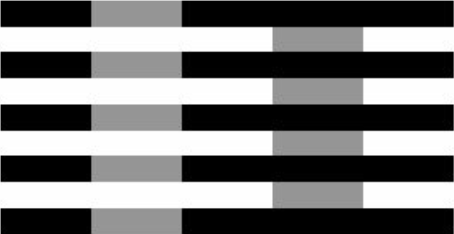
\includegraphics[width=\columnwidth, height=2cm]{images/Introduction/perc_intensity.png} 
				The gray fields have the same intensity (same gray tone).
			\end{flushleft}
		\end{minipage}
		\begin{minipage}[t]{0.49\columnwidth}
			\begin{flushright}
				{\centering Perception of \textbf{color}\\}
				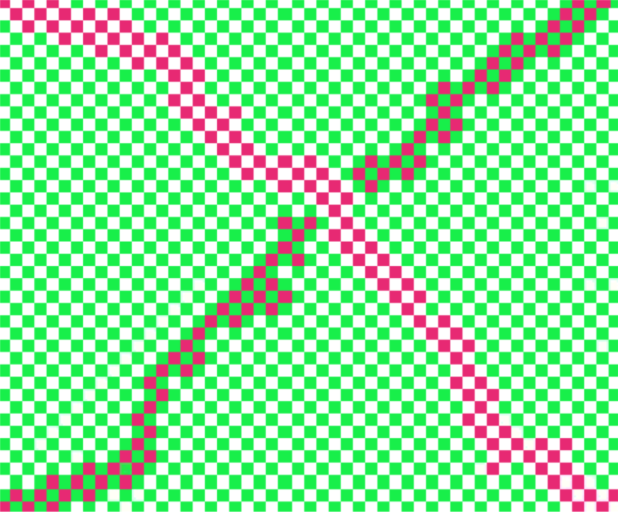
\includegraphics[width=\columnwidth, height=2cm]{images/Introduction/perc_color.png}
				The red squares have equal color
			\end{flushright}
		\end{minipage}
		\hrule
		\begin{minipage}[t]{0.49\columnwidth}
			\begin{flushleft}
				{\centering Perception of \textbf{length}\\}
				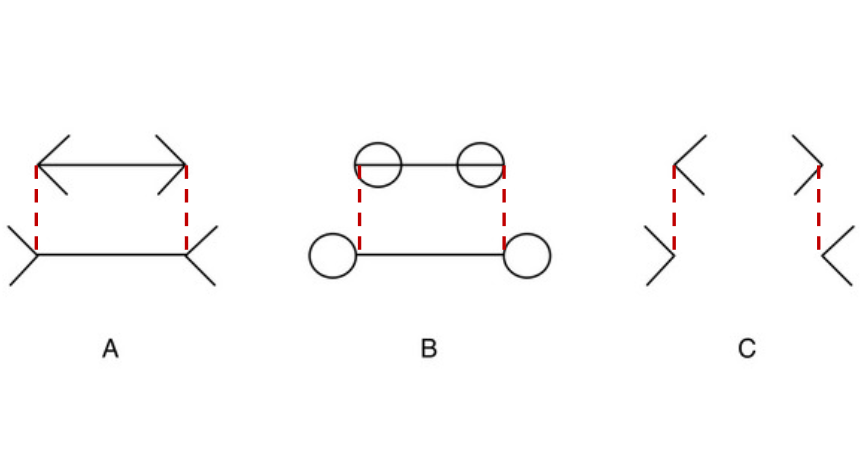
\includegraphics[width=\columnwidth, height=2cm]{images/Introduction/perc_length.png} 
				the horizontal lines are equally long.
			\end{flushleft}
		\end{minipage}
		\begin{minipage}[t]{0.49\columnwidth}
			\begin{flushright}
				{\centering \textbf{Lines being straight}
				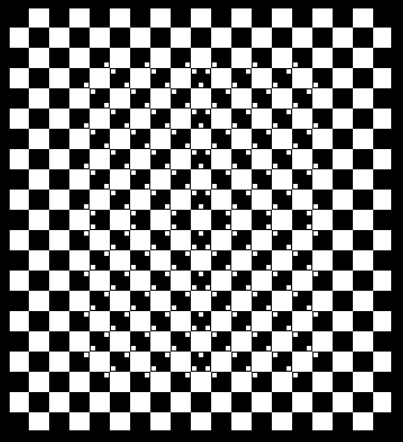
\includegraphics[width=2cm, height=2cm]{images/Introduction/perc_straight.png}\\}
				The lines do not have any curvature
			\end{flushright}
		\end{minipage}	
		\hrule
		\begin{minipage}[t]{0.49\columnwidth}
			\begin{flushleft}
				{\centering Perception of \textbf{parallelism}\\}
				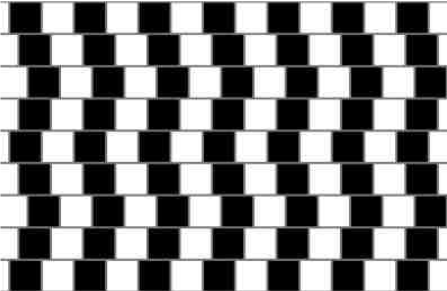
\includegraphics[width=\columnwidth, height=2cm]{images/Introduction/perc_parallel.png} 
				All lines are parallel.
			\end{flushleft}
		\end{minipage}
		\begin{minipage}[t]{0.49\columnwidth}
			\begin{flushright}
				{\centering Perception of \textbf{curvatures}
				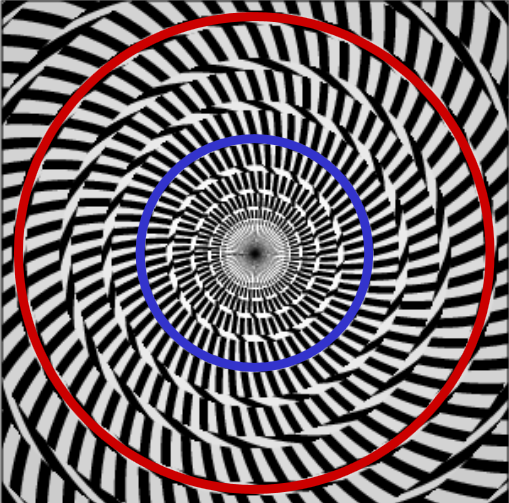
\includegraphics[width=2cm, height=2cm]{images/Introduction/perc_curvature.png}\\}
				There is no spiral.
			\end{flushright}
		\end{minipage}
		\begin{minipage}[t]{0.49\columnwidth}
			\begin{flushleft}
				{\centering Perception of \textbf{motion}\\}
				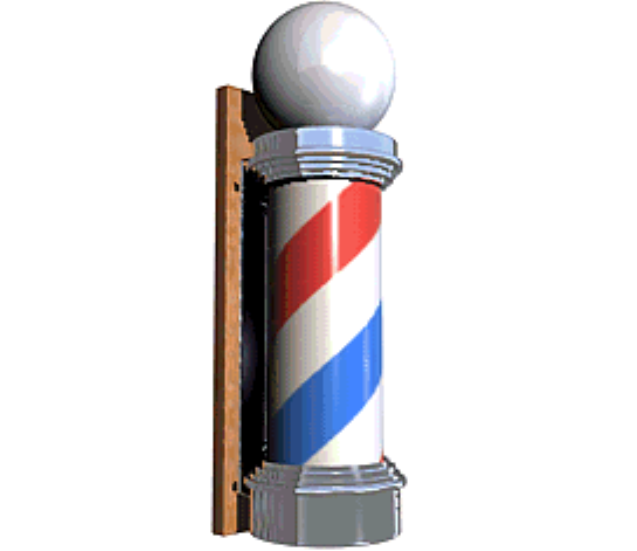
\includegraphics[width=\columnwidth, height=3cm]{images/Introduction/perc_motion.png} 
				The pole rotates about the vertical, it does not translate vertically.
			\end{flushleft}
		\end{minipage}
		\begin{minipage}[t]{0.49\columnwidth}
		\begin{flushright}
				{\centering The role of \textbf{context}
				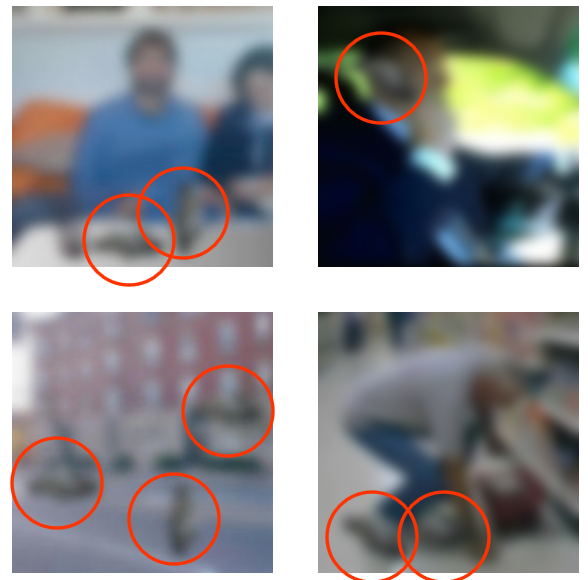
\includegraphics[width=3cm, height=3cm]{images/Introduction/perc_context.png}\\}
				All encircled patterns are identical!
			\end{flushright}
		\end{minipage}
		\par 
		\textcolor{red}{Take home message}:\\
		\textbf{\textcolor{red}{Effective vision needs more than sheer filtering and measuring}}
		\subsection{Applications}
		Most early applications where found in \textbf{production environments}, as these allow for \textbf{controlled conditions} and have \textbf{little uncertainty}. But some areas do not allow for much control: medical IP, remote sensing, surveillance, etc.\\
		Currently Computer Vision (CV) is conquering the less controllable areas by storm:
		\par  
		\begin{minipage}[t]{0.49\columnwidth}
			\begin{flushleft}
		 		{\centering \textbf{Image enhancement:} mobile $\rightarrow$ DSLR\\}
		 		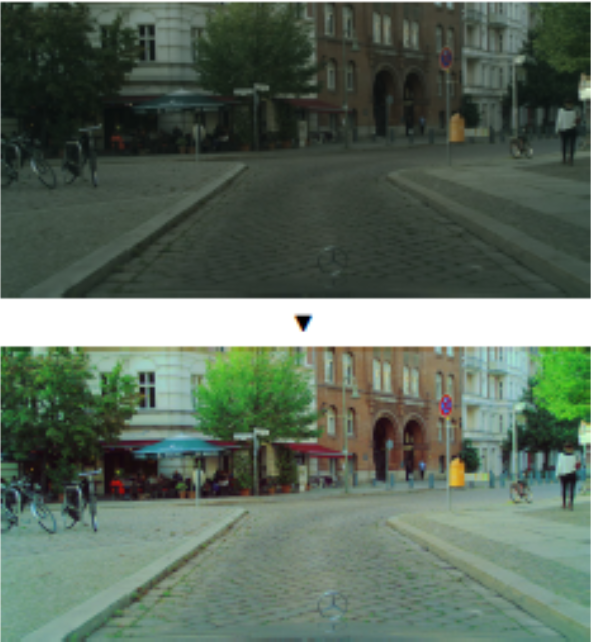
\includegraphics[width=\columnwidth, height=5cm]{images/Introduction/app_enhancement.png} 
			\end{flushleft}
		\end{minipage}
		\begin{minipage}[t]{0.49\columnwidth}
			\begin{flushright}
				{\centering \textbf{Image retrieval, captioning}\\}
				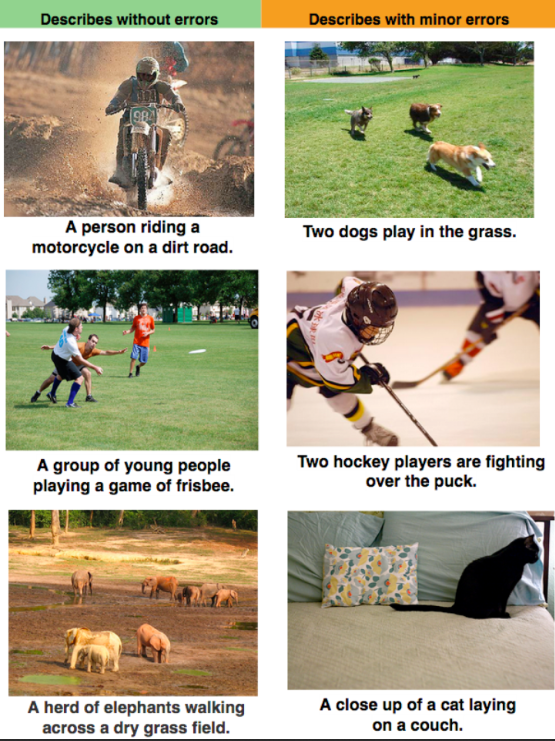
\includegraphics[width=\columnwidth, height=5cm]{images/Introduction/app_retrieval.png}
			\end{flushright}
		\end{minipage}
		\hrule
		\begin{minipage}[t]{0.49\columnwidth}
			\begin{flushleft}
				{\centering \textbf{Autonomous vehicles}\\}
				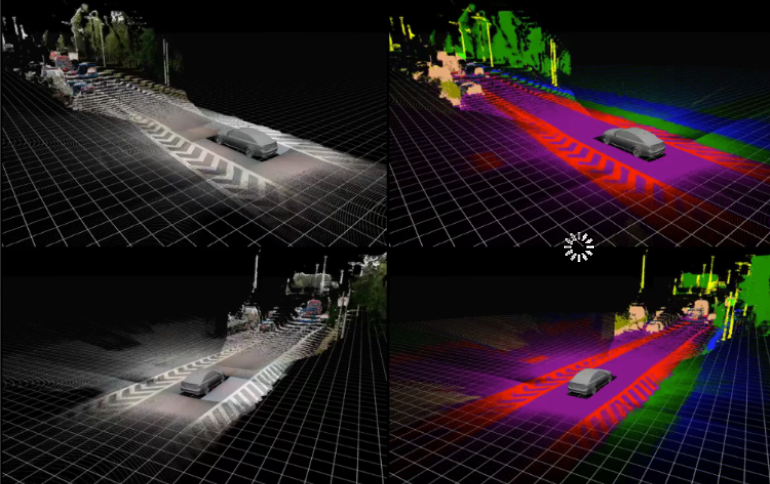
\includegraphics[width=\columnwidth, height=3cm]{images/Introduction/app_autonomous_vehicles.png} 
			\end{flushleft}
		\end{minipage}
		\begin{minipage}[t]{0.49\columnwidth}
			\begin{flushright}
				{\centering \textbf{Visual surveillance}\\}
				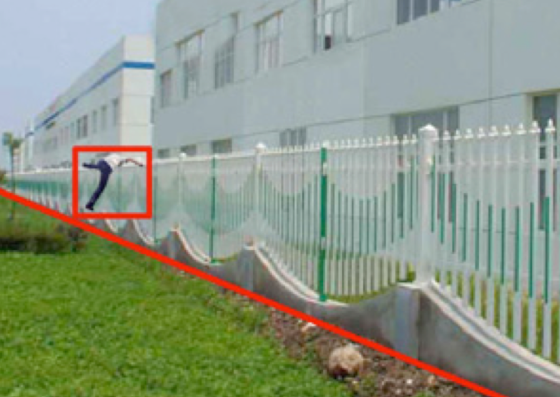
\includegraphics[width=\columnwidth, height=3cm]{images/Introduction/app_surveillance.png}
			\end{flushright}
		\end{minipage}
		\hrule
		\begin{minipage}[t]{0.49\columnwidth}
			\begin{flushleft}
				{\centering \textbf{Augmented Reality, e.g sports}\\}
				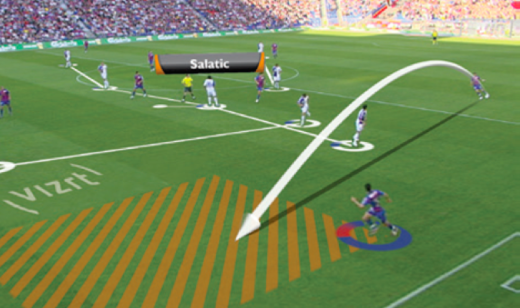
\includegraphics[width=\columnwidth, height=2.5cm]{images/Introduction/app_augm_reality.png} 
			\end{flushleft}
		\end{minipage}
		\begin{minipage}[t]{0.49\columnwidth}
			\begin{flushright}
				{\centering \textbf{Computer-assisted surgery}\\}
				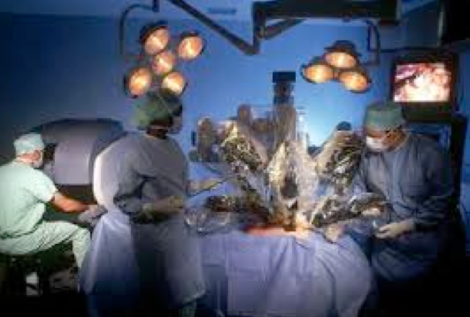
\includegraphics[width=\columnwidth, height=2.5cm]{images/Introduction/app_surgery.png}
			\end{flushright}
		\end{minipage}			
		\par 
		\textcolor{red}{Take home message}:\\
		\textbf{\textcolor{red}{It is feasible now to let most things see and interpret their environment.}}
		
		\subsection{The nature of light}
		There are three different models to describe optical systems: 
		\begin{enumerate}[noitemsep]
			\item Geometrical optics
			\item Physical optics $\rightarrow$ \textcolor{red}{\textbf{wave character}}   
			\item Quantum-mechanical optics
		\end{enumerate}
		In this course we mainly look at physical optics and the wave character of light. 		
		\subsubsection{Light as EM-waves}
		Self-sustaining exchange of electric and magnetic fields. An EM-wave is characterized with the following properties: 
		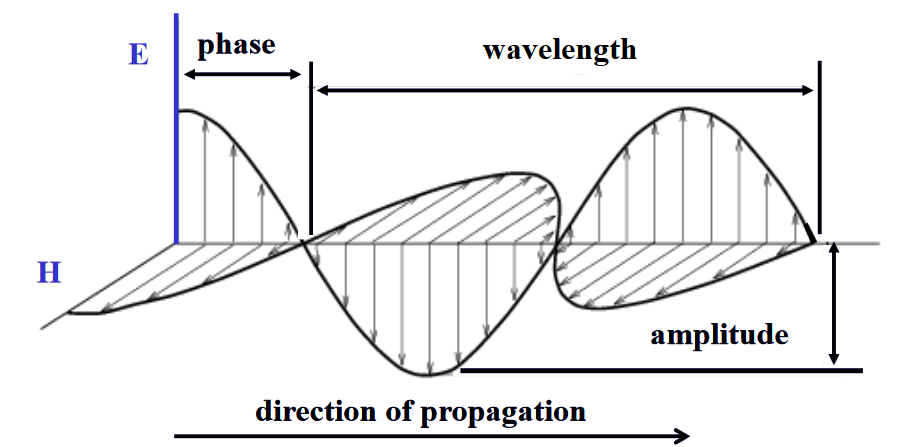
\includegraphics[width=\columnwidth]{images/Introduction/em_wave.png}			
			\begin{itemize}[noitemsep]
				\item \textbf{Wavelength}
				\item Direction of \textbf{propagation}
				\item \textbf{Amplitude} of E
				\item \textbf{Phase} 
				\item Direction of \textbf{polarization }
			\end{itemize}
		\textbf{The spectrum:}\\
		Normal ambient light is a mixture of wavelengths, polarization directions and phases. The visible range for humans is only a small fraction of the EM-waves-spectrum.\\
		\begin{center}
			\begin{tabular}{c l l}
				\hline 
				\hline
				Wavelength [$nm$] &  & Color \\ 
				\hline 
				380 - 450 & $\rightarrow$ & \textcolor{violet}{violet} \\ 
				450 - 490 & $\rightarrow$ & \textcolor{blue}{blue} \\ 
				490 - 560 & $\rightarrow$ & \textcolor{green}{green} \\ 
				560 - 590 & $\rightarrow$ & \textcolor{yellow}{yellow} \\ 
				590 - 630 & $\rightarrow$ & \textcolor{orange}{orange} \\ 
				630 - 760 & $\rightarrow$ & \textcolor{red}{red} \\
				\hline
				\hline 
			\end{tabular}
		\end{center}
		%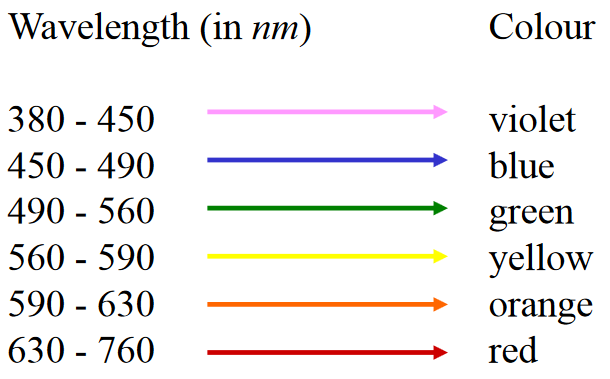
\includegraphics[height=3cm]{images/Introduction/visible_spectrum.png}
		The visible range differs from humans to animals and also cameras may have different spectral sensitivities. There are also cameras for non-visible light such as infrared. The following picture shows the three color cones humans have and their sensitivity range: 
		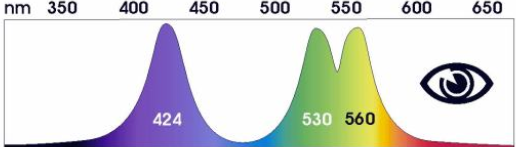
\includegraphics[width=\columnwidth]{images/Introduction/human_cones.png}
		  
		\subsubsection{Interactions with matter}
		We look at the following types of interaction with matter: 
		\begin{enumerate}[noitemsep]
			\item \textbf{Absorption}
				\begin{itemize}[label={$\rightarrow$}]
					\item blue water
				\end{itemize}
			\item \textbf{Scattering}
				\begin{itemize}[label={$\rightarrow$}]
					\item blue sky
					\item red sunset
				\end{itemize}
			\item \textbf{Reflection}
				\begin{itemize}[label={$\rightarrow$}]
					\item colored ink
				\end{itemize} 
			\item \textbf{Refraction}
				\begin{itemize}[label={$\rightarrow$}]
					\item dispersion by a prism
				\end{itemize} 
			\item \textbf{Diffraction} 
		\end{enumerate}
		 We look at few of those in more detail:
		 \par
		  
		 \textbf{1. Absorption}\\
		 A nice example of absorption is earth's atmosphere which absorbs certain wavelengths of the incoming light. The absorbed frequencies correspond to resonance frequencies of molecules in earth's atmosphere.\\ 
		 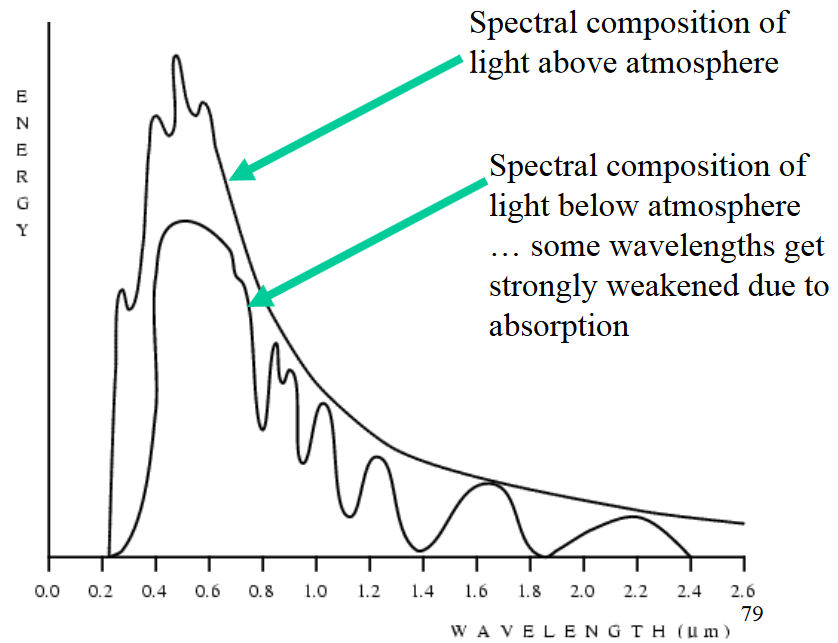
\includegraphics[width=\columnwidth]{images/Introduction/absorption_earth.png}
		 \clearpage 
		 
		 \textbf{2. Scattering}\\
		 There are three types of scattering depending on the relative sizes of particles and wavelengths:
		 \begin{enumerate}[label=(\alph*)]
		 	\item Small particles: \textcolor{red}{\textbf{Rayleigh}} (strong wavelength dependent)
		 	\item Comparable size: \textcolor{red}{\textbf{Mie}} (weakly wavelength dependent)
		 	\item Large particles: \textcolor{red}{\textbf{Non-selective}} (wavelength independent)
		 \end{enumerate}
	 	If we look at the scattered energy it looks as follows:\\ 
	 	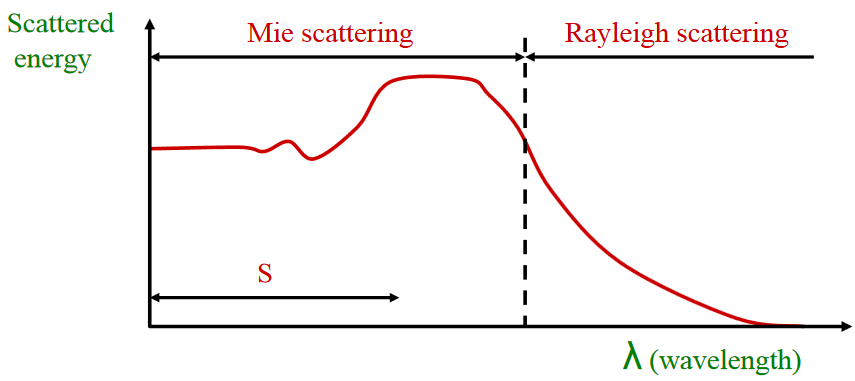
\includegraphics[width=\columnwidth]{images/Introduction/scattered_energy.png}
	 	
	 	Let's see some examples of these different scatter-types in our atmosphere:\\ 
	 	\begin{minipage}[t]{0.49\columnwidth}
	 		\begin{flushleft}
	 			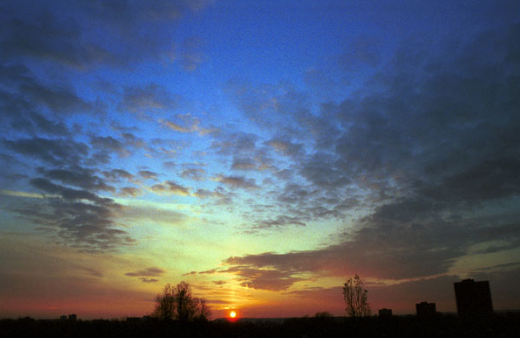
\includegraphics[width=\columnwidth]{images/Introduction/ex_ray_non.png}\\
	 		\end{flushleft}
	 	\end{minipage}
	 	\begin{minipage}[b]{0.49\columnwidth}
	 		\begin{flushleft}
	 			\textbf{Rayleigh}: Tyndall effect (blue sky, red setting sun)\\
	 			\textbf{Non-selective}: Grey clouds
	 		\end{flushleft}
	 	\end{minipage}
 		%\hrule
 		\par 
 		\begin{minipage}[t]{0.49\columnwidth}
 			\begin{flushleft}
 				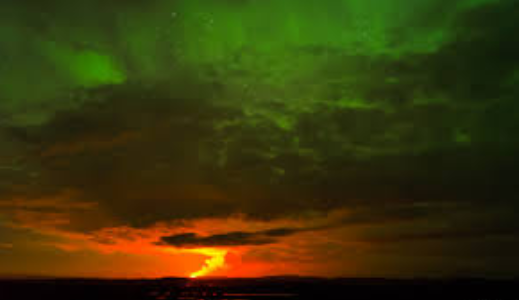
\includegraphics[width=\columnwidth]{images/Introduction/ex_mie.png}\\
 			\end{flushleft}
 		\end{minipage}
 		\begin{minipage}[b]{0.49\columnwidth}
 			\begin{flushleft}
 				\textbf{Mie}: Colored cloud from volcanic eruption
 				\vspace{0.6cm}
 			\end{flushleft}
 		\end{minipage}
		\par 
		\textbf{3. Reflection:}\\
		In mirror reflection we have:\\ angle of reflection = angle of incident.\\
		Two different categories of reflective materials:\\
		\begin{minipage}[t]{0.49\columnwidth}
			\begin{flushleft}
				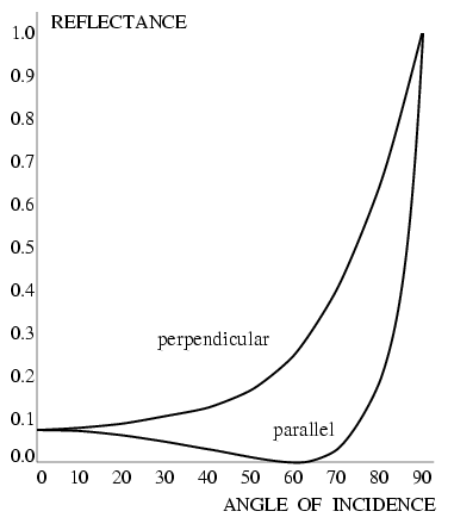
\includegraphics[width=\columnwidth]{images/Introduction/refl_diel.png}\\
			\end{flushleft}
		\end{minipage}
		\begin{minipage}[b]{0.49\columnwidth}
			\begin{flushleft}
				\textbf{Dielectric:}\\
				For parallel polarization there exists the Brewster angle where $r=0$.
				\vspace{1.2cm}
			\end{flushleft}
		\end{minipage}
		\par 
		\begin{minipage}[t]{0.49\columnwidth}
			\begin{flushleft}
				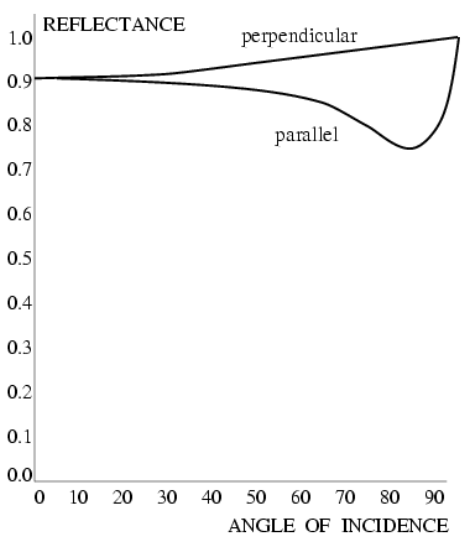
\includegraphics[width=\columnwidth]{images/Introduction/refl_metal.png}\\
			\end{flushleft}
		\end{minipage}
		\begin{minipage}[b]{0.49\columnwidth}
			\begin{flushleft}
				\textbf{Conductor:}\\
				Strong reflectors under all angles, more or less preserve polarization.
				\vspace{1.2cm}
			\end{flushleft}
		\end{minipage}
	
		We differentiate three types of reflection which depend on the surface structure: 
		\begin{minipage}[t]{0.49\columnwidth}
			\begin{flushleft}
				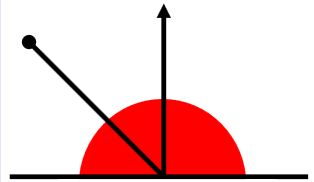
\includegraphics[width=\columnwidth]{images/Introduction/refl_diffuse.png}\\
			\end{flushleft}
		\end{minipage}
		\begin{minipage}[b]{0.49\columnwidth}
			\begin{flushleft}
				\textbf{Diffuse:}\\
				Also called \textbf{Lambertian}. Rough surfaces.
				\vspace{0.2cm}
			\end{flushleft}
		\end{minipage}
		\par
		\begin{minipage}[t]{0.49\columnwidth}
			\begin{flushleft}
				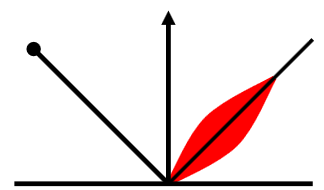
\includegraphics[width=\columnwidth]{images/Introduction/refl_mirror.png}\\
			\end{flushleft}
		\end{minipage}
		\begin{minipage}[b]{0.49\columnwidth}
			\begin{flushleft}
				\textbf{Specular:}\\
				Mirror-like surfaces.
				\vspace{0.5cm}
			\end{flushleft}
		\end{minipage}
		\par 
		\begin{minipage}[t]{0.49\columnwidth}
			\begin{flushleft}
				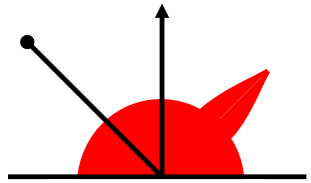
\includegraphics[width=\columnwidth]{images/Introduction/refl_mixed.png}\\
			\end{flushleft}
		\end{minipage}
		\begin{minipage}[b]{0.49\columnwidth}
			\begin{flushleft}
				\textbf{Mixed:}\\
				Mix of diffuse and specular.
				\vspace{0.5cm}
			\end{flushleft}
		\end{minipage}
		\par 
		\textbf{4. Refraction:}\\
		\begin{minipage}[t]{0.39\columnwidth}
			\begin{flushleft}
				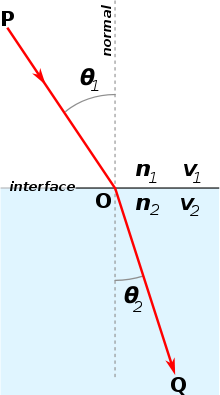
\includegraphics[width=\columnwidth]{images/Introduction/snells_law.png}\\
			\end{flushleft}
		\end{minipage}
		\begin{minipage}[b]{0.59\columnwidth}
			\begin{flushleft}
				Effect of the bending of light if it hits an interface of two materials with different refraction index $n=\sqrt{\epsilon\mu}$. The bending is described through \textbf{\textcolor{red}{Snell's law}}:\\
				%\vspace{0.2cm}
				\ceqbox{n_1\sin\theta_1=n_2\sin\theta_2}
				\vspace{1.1cm}
			\end{flushleft}
		\end{minipage}
		\par 
		\begin{minipage}[t]{0.49\columnwidth}
			\begin{flushleft}
				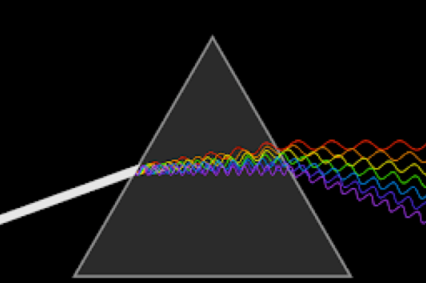
\includegraphics[width=\columnwidth]{images/Introduction/dispersion.png}\\
			\end{flushleft}
		\end{minipage}
		\begin{minipage}[b]{0.49\columnwidth}
			\begin{flushleft}
				\textbf{Dispersion:}\\
				The bending is dependent of the frequency (wavelength) of the light. 
				\vspace{0.2cm}
			\end{flushleft}
		\end{minipage}
		\vfill\null
		\columnbreak

		\section{Image Acquisition}	
		\subsection{Illumination}
		Well designed illumination often is key in visual inspection and can extremely simplify the image processing. Here is an overview of different illumination techniques:
		
		\subsubsection{Back-lighting}
		\begin{center}
			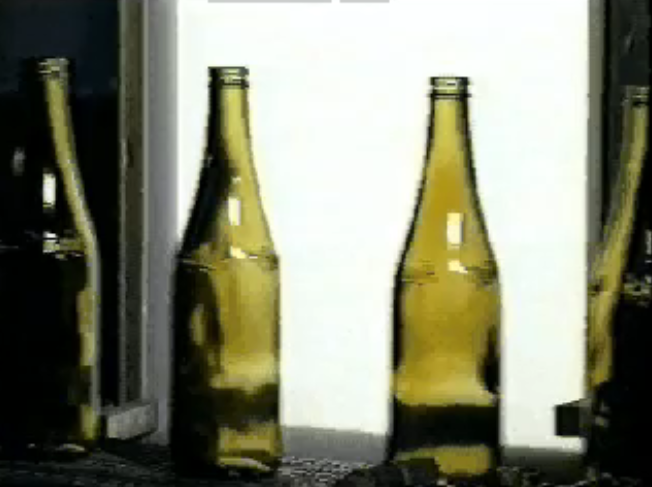
\includegraphics[width=0.7\columnwidth,]{images/ImageAcq/back_lighting.png}\\
		\end{center}
		
		\textbf{How:}\\
		Lamps are placed behind a transmitting diffuser plate which is located behind the object
		\par 
		\textbf{Why:}\\
		Creates \textbf{high-contrast} silhouette images, easy to handle with \textbf{binary vision} (only two intensity levels, black and white). Often used in inspection.
	
		\subsubsection{Directional-lighting}
		\begin{center}
			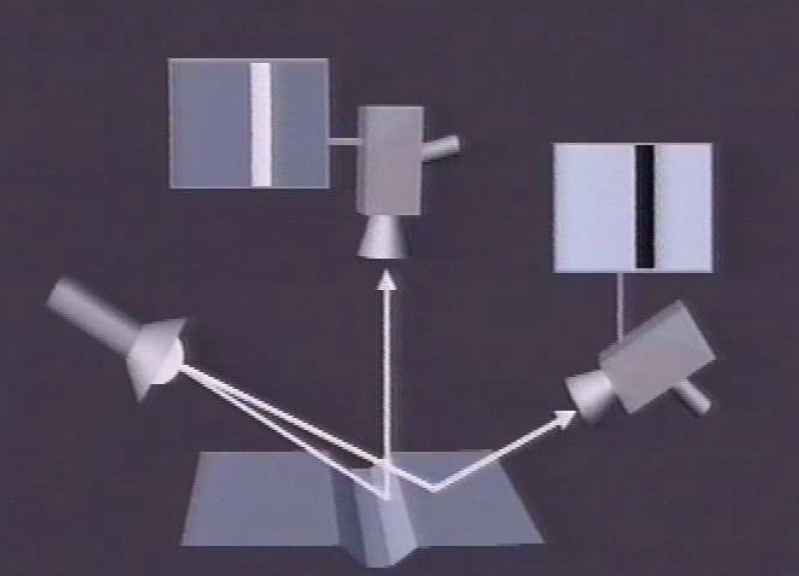
\includegraphics[width=0.7\columnwidth,]{images/ImageAcq/directional_lighting.png}\\
		\end{center}
	
		\textbf{How:}\\
		Light source shines directly on object, maybe under a certain angle.
		\par 
		\textbf{Why:}\\
		\vspace{-0.5cm}
		\begin{itemize}[noitemsep]
			\item Generation of \textbf{specular reflection} (e.g. crack detection (see figure above))
			\item Generation of \textbf{sharp shadows}
		\end{itemize}
		\vfill\null
		\columnbreak
		
		\subsubsection{Diffuse-lighting}
		\begin{minipage}[t]{0.49\columnwidth}
			\begin{flushleft}
				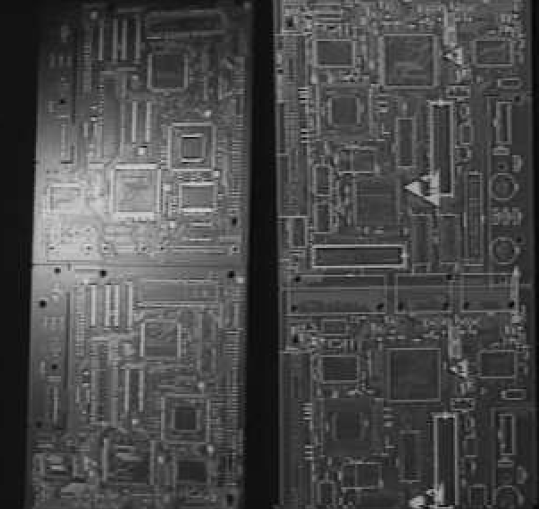
\includegraphics[width=\columnwidth]{images//ImageAcq/diffusive_lighting.png}\\
			\end{flushleft}
		\end{minipage}
		\begin{minipage}[b]{0.49\columnwidth}
			\begin{flushleft}
				\textbf{Left:}\\
				Direct lighting produced large changes in brightness due to specular reflection.\\
				\vspace{0.2cm}
				\textbf{right:}\\
				Diffusive lighting reduces bright spots. 
				\vspace{0.2cm}
			\end{flushleft}
		\end{minipage}
	
		\textbf{How:}\\
		Do not directly shine with light source on object, but rather indirectly with the help of a diffusive surface. It does not reduces the specular reflection, but increases the diffuse reflection component, yielding in less variations.
		\par 
		\textbf{Why:}\\
		Prevents sharp shadows and large intensity variations over glossy surface.  
	
		\subsubsection{Polarized-lighting}
		The polarization direction is the one of the E-Wave. Normally, light is composed of many waves with different polarizations. \\
		Following picture shows a polarizer/analyzer configuration:\\
		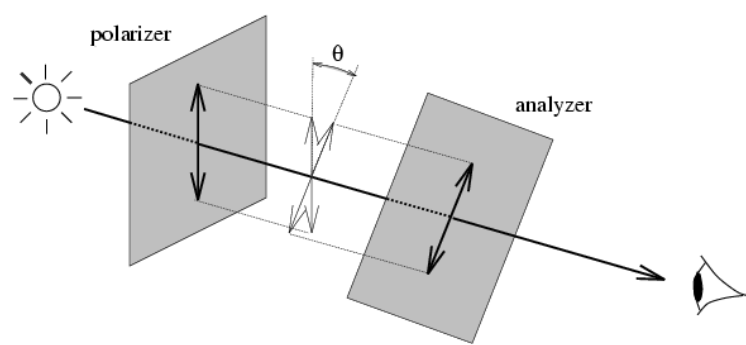
\includegraphics[width=\columnwidth]{images//ImageAcq/polarizer_analyzer.png}
		The intensity seen from the observer depends on the angle $\theta$ and is described by the \textcolor{red}{\textbf{law of Malu}s}:\\
		\ceqbox{I(\theta)=I(0)\cos^2\theta}
		There are 2 uses for polarized lighting:
		\begin{enumerate}[noitemsep]
			\item Improve contrast between Lambertian and specular reflection.
			\item Improve contrast between dielectrics and metals.
		\end{enumerate}
		\vfill\null
		\columnbreak
		
		\textbf{1. Specular vs. Lambertian}\\
		\begin{center}
			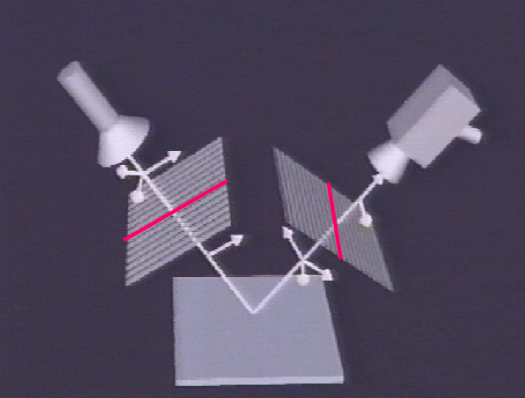
\includegraphics[width=0.7\columnwidth]{images//ImageAcq/diffuse_specular.png}\\
		\end{center}
		\textbf{How:}\\
		Polarizer and analyzer in crossed arrangement. Specular reflection keeps polarization, Lambertian reflection depolarizes, because of this the arrangement reduces the large dynamic range caused by glare. 
		\par 
		\textbf{Why:}\\
		Increases contrast between Lambertian and specular reflection (specular reflection gets blocked).
		
		\textbf{2. Dielectric vs. Metal}\\
		\begin{center}
			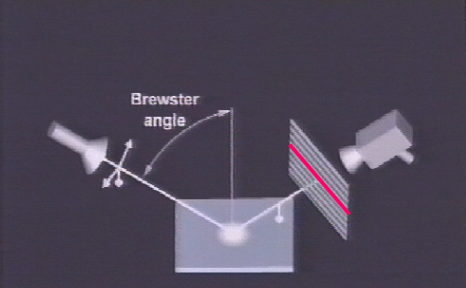
\includegraphics[width=0.7\columnwidth]{images//ImageAcq/dielectric_metal.png}\\
		\end{center}
		\textbf{How:}\\
		Shine non-polarized light at Brewster angle on object. The dielectric will not reflect the parallel polarized component (Brewster angle...) and the perpendicular component is filtered out by the analyzer, hence the dielectric parts of the object will be really dark.  
		\par 
		\textbf{Why:}\\
		Increases contrast between dielectrics and metals (dielectric reflection gets blocked).
		\vfill\null
		\columnbreak
		
		\subsubsection{Colored-lighting}
		\begin{minipage}[t]{0.49\columnwidth}
			\begin{flushleft}
				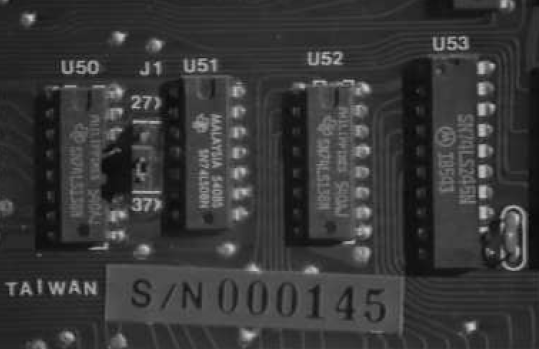
\includegraphics[width=\columnwidth]{images//ImageAcq/white_light.png}\\
			\end{flushleft}
		\end{minipage}
		\begin{minipage}[b]{0.49\columnwidth}
			\begin{flushleft}
				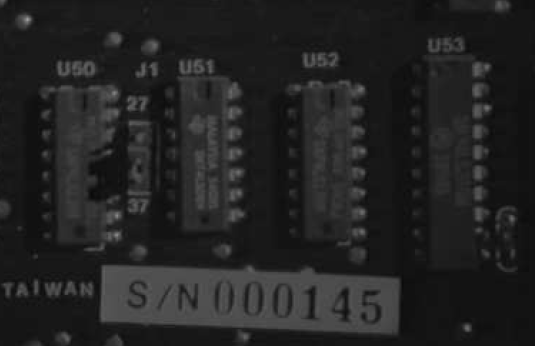
\includegraphics[width=\columnwidth]{images//ImageAcq/red_light.png}\\
			\end{flushleft}
		\end{minipage}
		The contrast between the red label and the green PCB is increased when red light is shined on it (right) in comparison to white light (left).\\
		\par 
		\textbf{How:}\\
		Shine colored light at an object and maybe also use an bandpass filter. You need to have in mind the spectral sensitivity of your sensor!
		\par 
		\textbf{Why:}\\
		\vspace{-0.5cm}
		\begin{itemize}[noitemsep]
			\item Highlight regions of similar color
			\item Differentiate between specular and diffuse reflection
			\item Comparing color
		\end{itemize}
		
		\subsubsection{Structures-lighting}
		\begin{center}
			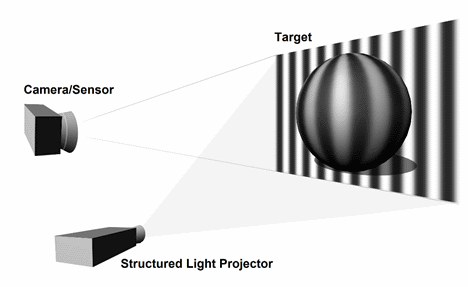
\includegraphics[width=0.7\columnwidth]{images//ImageAcq/structured_lighting.png}\\
		\end{center}
		\textbf{How:}\\
		Spatially or temporally modulated light patterns are shined on a 3D object.
		\par 
		\textbf{Why:}\\
		Obtain 3D info of object.
		\par
		More on this later...
	
		\subsubsection{Stroboscopic-lighting}
		\begin{minipage}[t]{0.49\columnwidth}
			\begin{flushleft}
				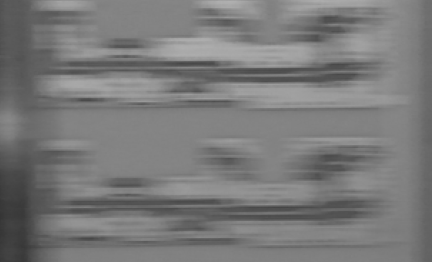
\includegraphics[width=\columnwidth, height=2cm]{images//ImageAcq/blur.png}\\
			\end{flushleft}
		\end{minipage}
		\begin{minipage}[t]{0.49\columnwidth}
			\begin{flushleft}
				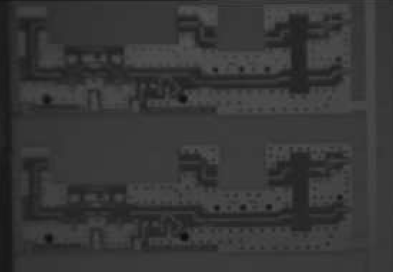
\includegraphics[width=\columnwidth, height=2cm]{images//ImageAcq/no_blur.png}\\
			\end{flushleft}
		\end{minipage}
		\par 
		\textbf{How:}\\
		High intensity light flashes. The light flash artificially shortens the sensors integration time. Mostly this is much cheaper than fast cameras.
		\par 
		\textbf{Why:}\\
		Eliminate motion blur
		
		\subsection{Cameras}
		\subsubsection{Camera models}
		\textbf{Pinhole-model}\\
		\begin{minipage}[b]{0.49\columnwidth}
			\begin{flushleft}
				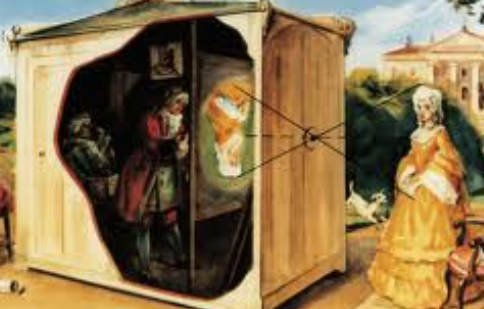
\includegraphics[width=\columnwidth, height=2cm]{images//ImageAcq/pinhole_1.png}\\
			\end{flushleft}
		\end{minipage}
		\begin{minipage}[t]{0.49\columnwidth}
			\begin{flushleft}
				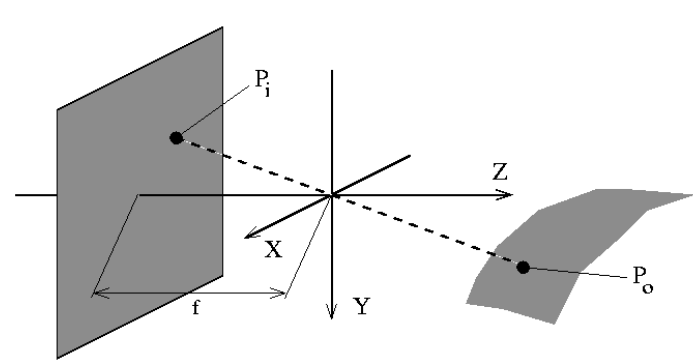
\includegraphics[width=\columnwidth, height=2cm]{images//ImageAcq/pinhole_2.png}\\
			\end{flushleft}
		\end{minipage}
		Light enters the box only through a small hole and an image is formed on a plane inside the box. If the whole is too small not enough light enters and additional diffraction occurs, if the whole is too big, the image gets blurry. The solution to this problem is a lens. From similar triangles the following formula follows:
		\begin{center}
			$\dfrac{X_i}{X_o}=\dfrac{Y_i}{Y_o}=\dfrac{f}{Z_o}=-m=$ \textit{linear magnification}\\
		\end{center}
		\vspace{0.5cm}
		\textbf{The thin-lens model}\\
		\begin{center}
			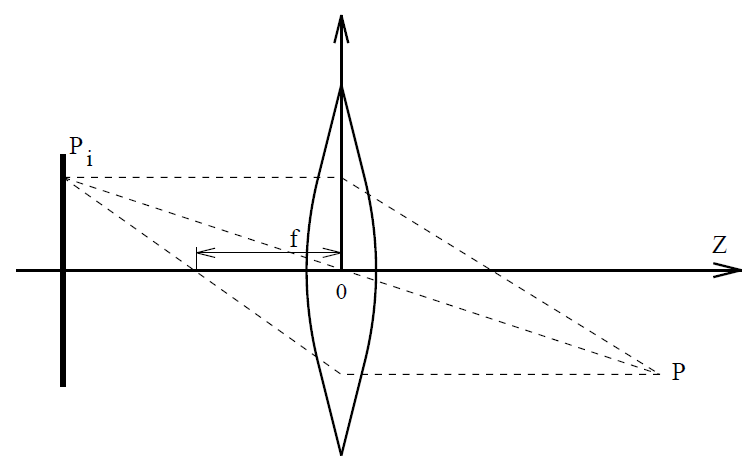
\includegraphics[width=0.7\columnwidth]{images//ImageAcq/thin_lens.png}\\
		\end{center}
		A lens captures more light and focuses it which gets rid off the problems of the pinhole. The price we pay is that only points at certain plane will be sharply imaged. Similar to the pinhole model the \textcolor{red}{\textbf{thin lens equation}} reads as:
		\ceqbox{\dfrac{1}{Z_o}-\dfrac{1}{Z_i}=\dfrac{1}{f}}
		\par 
		\textbf{The depth-of-field}\\
		\begin{center}
			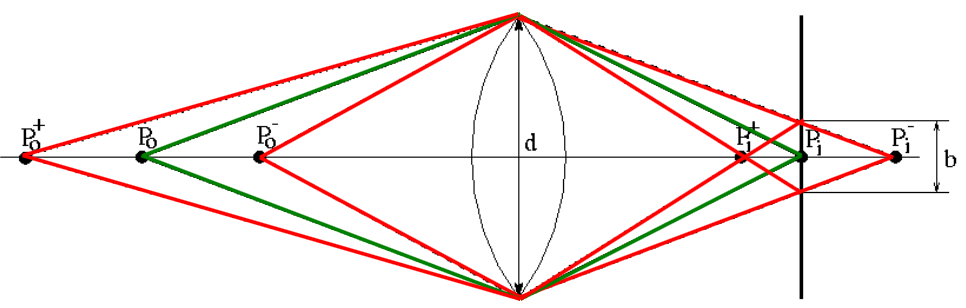
\includegraphics[width=0.7\columnwidth]{images//ImageAcq/depth_of_field.png}\\
		\end{center}
		As already mentioned only at a specific plane the image will be sharp, we can define an interval $\Delta Z_o^-$ in which we have a reasonable sharpness of the image:
		\begin{center}
			$\Delta Z_o^-=Z_o-Z_o^-=\dfrac{Z_o(Z_o-f)}{Z_o+fd/b-f}$\\
		\end{center}
		The depth-of-field \textbf{decreases with $\mathbf{d}$} and \textbf{increases with $\mathbf{Z_o}$}. The more we focus with the lens, the smaller the depth-of-field is, because de rays diverge stronger outside of the focal point. There is also a trade off between collecting a lot light (big $d$) and a large depth-of-field (usable depth range).
		\par 
		\textcolor{red}{Take home message}:\\
		\textbf{\textcolor{red}{In summary, introducing a lens to some extent solves the problem of insufficient light reaching the light detecting area of the camera. The price we pay is the loss of overall sharpness, i.e. points at a distance outside some range are no longer in focus.}}
		
		\subsubsection{Aberrations}
		In the above lens-model we made three assumptions:
		\begin{enumerate}[noitemsep]
			\item All rays from a point are focused onto 1 image point
			\item All image points in a single plane
			\item Magnification is constant
		\end{enumerate}
		Deviations form this ideal are called \textcolor{red}{\textbf{aberrations}}. We differentiate between two types of aberrations:
		\begin{enumerate}[noitemsep]
			\item \textbf{Geometrical}: visible as image distortions or degradation like blurring
				\begin{itemize}
					\item Spherical aberration
					\item astigmatism
					\item \textbf{radial distortion} (most important)
					\item coma
				\end{itemize}
			\item \textbf{Chromatic}: visible as different behavior for different wavelengths (color)
		\end{enumerate}
		
		\textbf{Spherical Aberration:}\\
		\begin{center}
			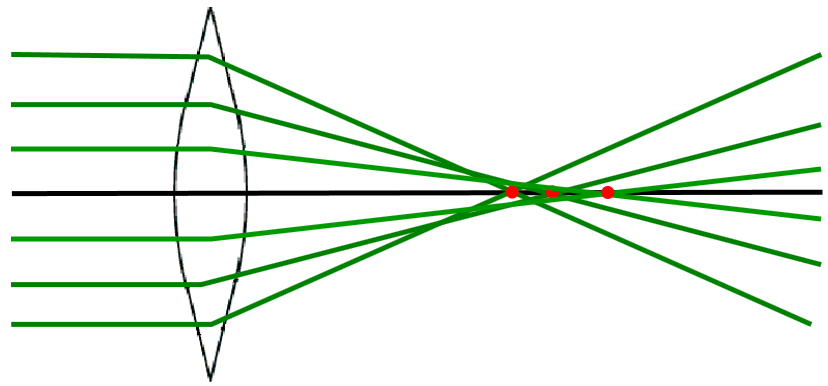
\includegraphics[width=0.7\columnwidth]{images//ImageAcq/spherical_aberration.png}\\
		\end{center}
		Rays parallel to the optical axis do not converge, because outer parts of the length yield smaller focal lengths. This results in blurry edges on the image.
		\begin{center}
			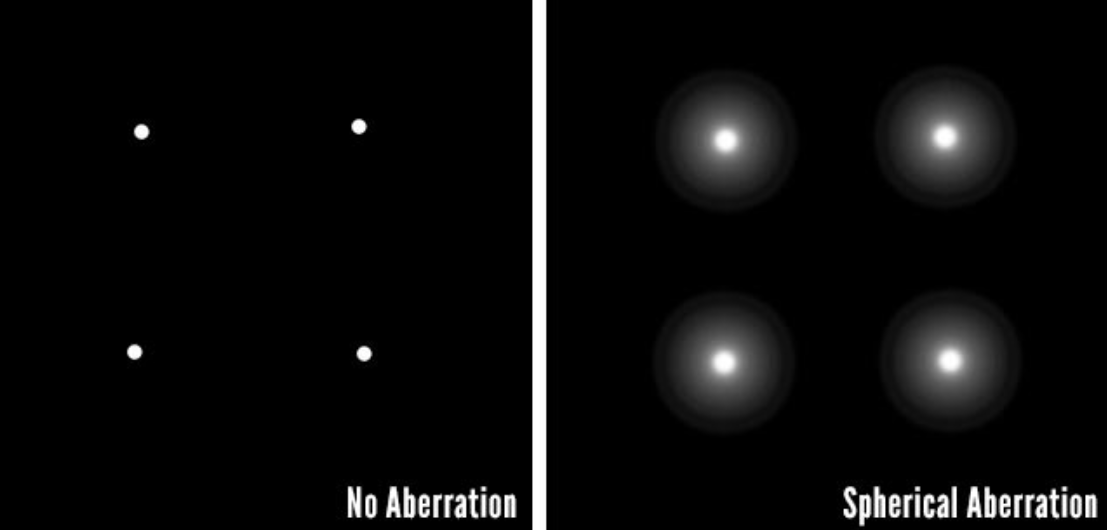
\includegraphics[width=0.7\columnwidth]{images//ImageAcq/spherical_aberration_2.png}\\
		\end{center}
		\vfill\null
		\columnbreak
		
		\textbf{Radial distortion:}\\
		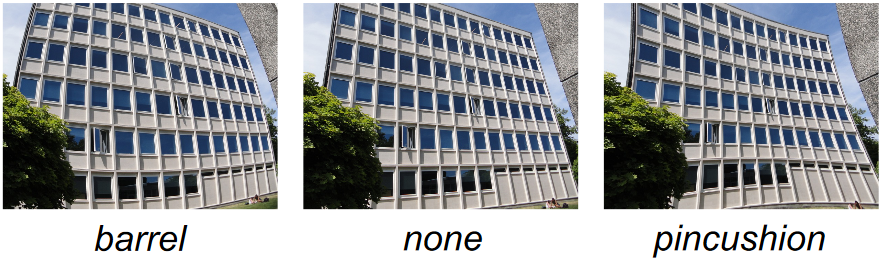
\includegraphics[width=\columnwidth]{images//ImageAcq/radial_dist.png}\\
		Different magnification for different angles of incident. This results in: 
		\begin{itemize}
			\item Lines become curves
				\begin{itemize}[label={$\rightarrow$}]
					\item Curvature increases as you move away form the center of distortion
						\begin{itemize}[label={$\rightarrow$}]
							\item Model assume this is the image center and there is a multiplicative factor on the pixel depending on the distance $r$ to the center:
							\vspace{-0.4cm}
							\ceqbox{d=1+\kappa_1r^2+\kappa_2r^4+\dots}
							Only even factors because effect is symmetric.\\
							This aberration can be corrected by software if the parameters $\kappa_1, \kappa_2, \dots$ are known.
						\end{itemize} 
				\end{itemize}
		\end{itemize}
		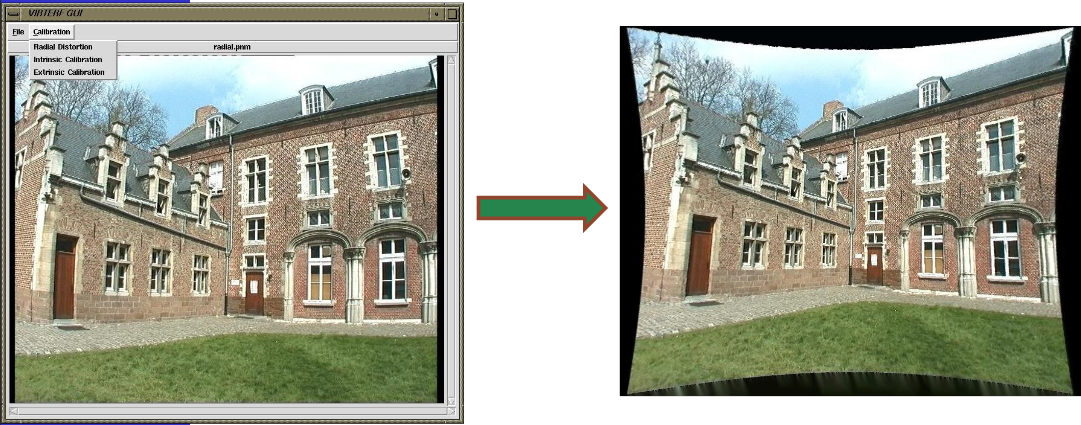
\includegraphics[width=\columnwidth]{images//ImageAcq/radial_dist_2.png}\\
		\par 
		\textbf{Chromatic distortion:}
		\begin{center}
			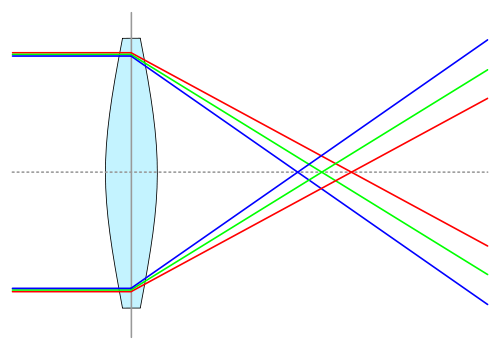
\includegraphics[width=0.7\columnwidth]{images//ImageAcq/chromatic_aberration.png}\\
		\end{center}
		Rays fo different wavelength focused on different planes. This can not be removed completely, but \textcolor{red}{\textbf{achromatization}} can be achieved at some well chosen wavelength pair, by combining lenses made of different glasses: 
		\begin{center}
			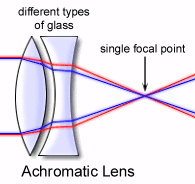
\includegraphics[width=0.7\columnwidth]{images//ImageAcq/achromatization.png}\\
		\end{center}
		Sometimes achromatization is achieved for more than two wavelengths. 
		
		\subsubsection{Device technologies}
		We consider 2 types: 
		\begin{center}
			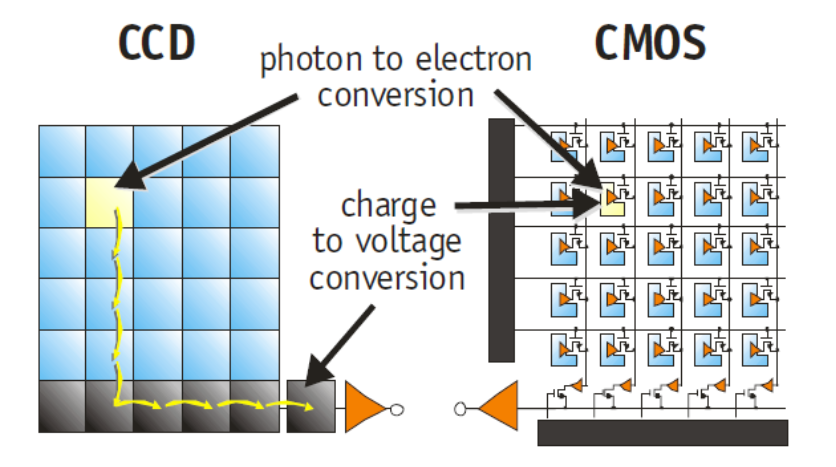
\includegraphics[width=0.7\columnwidth]{images//ImageAcq/ccd_cmos.png}\\
		\end{center}
		\begin{tabular}{l l}
			\hline 
			\hline
			\thead{CCD} &  \thead{CMOS}  \\ 
			\hline
			Niche applications    & Consumer cameras  \\ 
			Specific technology   & Standard IC technology\\ 
			Expensive product.	  & Cheap \\ 
			High power 			  & Low power \\ 
			Higher fill rate 	  & Less sensitive  \\ 
			Blooming			  & Per pixel amplif. \\ 
			Sequential readout	  & Random pixel access\\ 
								  & Smart pixels \\
								  & On chip with other comp.\\
			\hline 
			\hline
		\end{tabular}
		\par
		In 2006 was year of sales cross-over and in 2015 Sony said to stop CCD chip production. 
		\subsubsection{Color cameras}
		\subsubsection{Geometric models}
		\subsubsection{Photometric camera model}
		\section{Feature Extraction}	
		
		 
		
	\end{multicols*}
	\setcounter{secnumdepth}{3}
\end{document}
